\chapter{Analyse des FIR-Filters}
\section{Aufgabenstellung}
In dieser Aufgabe sollte zunächst die 3dB-Grenzfrequenz des Tiefpass-Filters ermittelt werden.
Im weiteren Verlauf sollte mithilfe des \gls{fda} - Tools ein IIR-Bandpass-Filter entworfen werden.
Folgende Charakteristik ist dabei zu erreichen:
\begin{itemize}
\item Butterworth-Charakteristik
\item Stoppband-Frequenzen: 2000Hz, 4000Hz
\item Passband-Frequenzen: 2000Hz, 4000Hz
\item Passband-Welligkeit: 1dB
\item Stoppband-Dämpfung: 60dB
\end{itemize}
\section{Durchf\"uhrung}
\subsection*{IIR-Tiefpass-Filter}
Zur Ermittlung der 3dB-Grenzfrequenz sollte die Frequenz so eingestellt werden, dass das Ausgangssignal 70\% der Amplitude des Ausgangssignals bei 50Hz entspricht.
Dafür wurde die Amplitude bei 50Hz auf 1V eingestellt, danach haben wir uns das Spektrum des Systems angeschaut.\\\par Dies ist in Abbildung \ref{fig:SprektrumZoomSystem} zu sehen. Dort sehen wir 3dB-Dämpfung bei 4060Hz. Dies entspricht den Erwartungen, da der Filter seine Grenzfrequenz bei ungefähr 4kHz haben sollte. 
\begin{figure}[H]
  \centering
    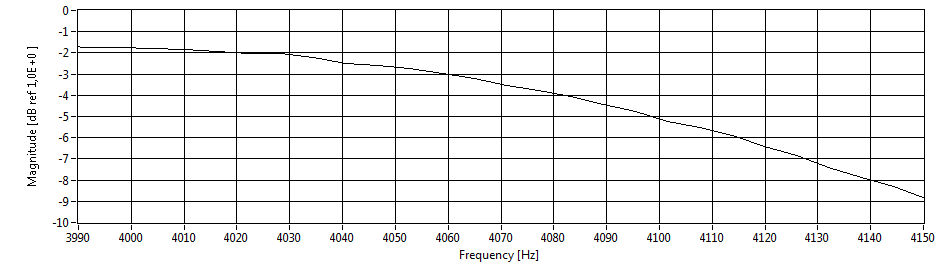
\includegraphics[width=\textwidth]{SpektrumEingezoomt.png}
  \caption{Ausschnitt des Spektrums des Systems}
  \label{fig:SprektrumZoomSystem}
\end{figure}


Im weiteren haben wir dann eine Aufnahme mit dem VI gemacht. Diese ist in Abbildung \ref{fig:4060HzScope} zu sehen, dieses Ergebnis war zu erwarten. Es ist zu sehen das das rote Ausgangssignal bei ungefähr 0,7V liegt und damit 70\% der ehemals 1V hat. Die Frequenz wurde auf 4060Hz eingestellt.
\begin{figure}[H]
  \centering
    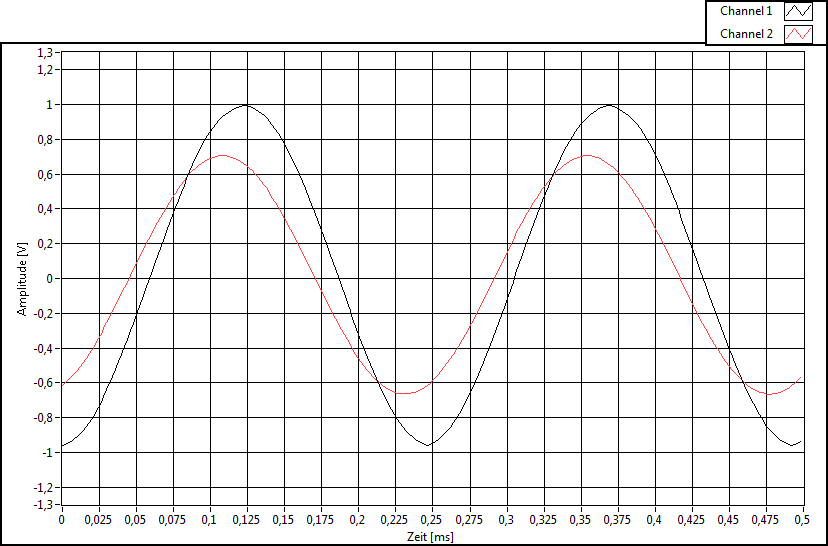
\includegraphics[width=\textwidth]{Sin1V_4,060kHz.png}
  \caption{Ein- und Ausgangssignal nebeneinander}
  \label{fig:4060HzScope}
\end{figure}

\subsection*{IIR-Bandpass-Filter}
Der zweite Teil behandelte die Erstellung IIR-Bandpass-Filters. Zu allererst mussten dafür die Koeffizienten generiert werden. Diese wurde dann mit Matlab abermals optimiert.
\lstinputlisting[title=Matlab-Code zur Optimierung der Koeffizienten]{OptimierungBandpass.m}

Die Berechnung erfolgte wie bereits für den Tiefpass-Filter. Anschließend mussten die Koeffizienten in den C-Code eingefügt werden.\\
\begin{adjustbox}{width=\textwidth, keepaspectratio} 
  \label{code:procdataKompFIR}
  \begin{lstlisting}[title=Codeausschnitt der modifizierten process\_data.c]
// Definition der Filterkoeffizienten
#define BIQUAD_STAGES 4 // Anzahl der Koeffizienten

const short coef[6*BIQUAD_STAGES] = {
	1,  -122,	   0,	 122, -16139, 30276, //H4
	1,  -651,      0,	 651, -16116, 29781, //H3
	1,  -343,      0,	 343, -15783, 29817, //H2
	1,  -451,	   0,	 451, -15760, 29601  //H1
};
  \end{lstlisting}
\end{adjustbox}

Zur Überprüfung der Implementierung wurde der Amplitudengang und die Sprungantwort aufgenommen. Diese wurden dann mit den von Matlab generierten Idealen Vorgaben verglichen.
\begin{figure}[H]
  \centering
    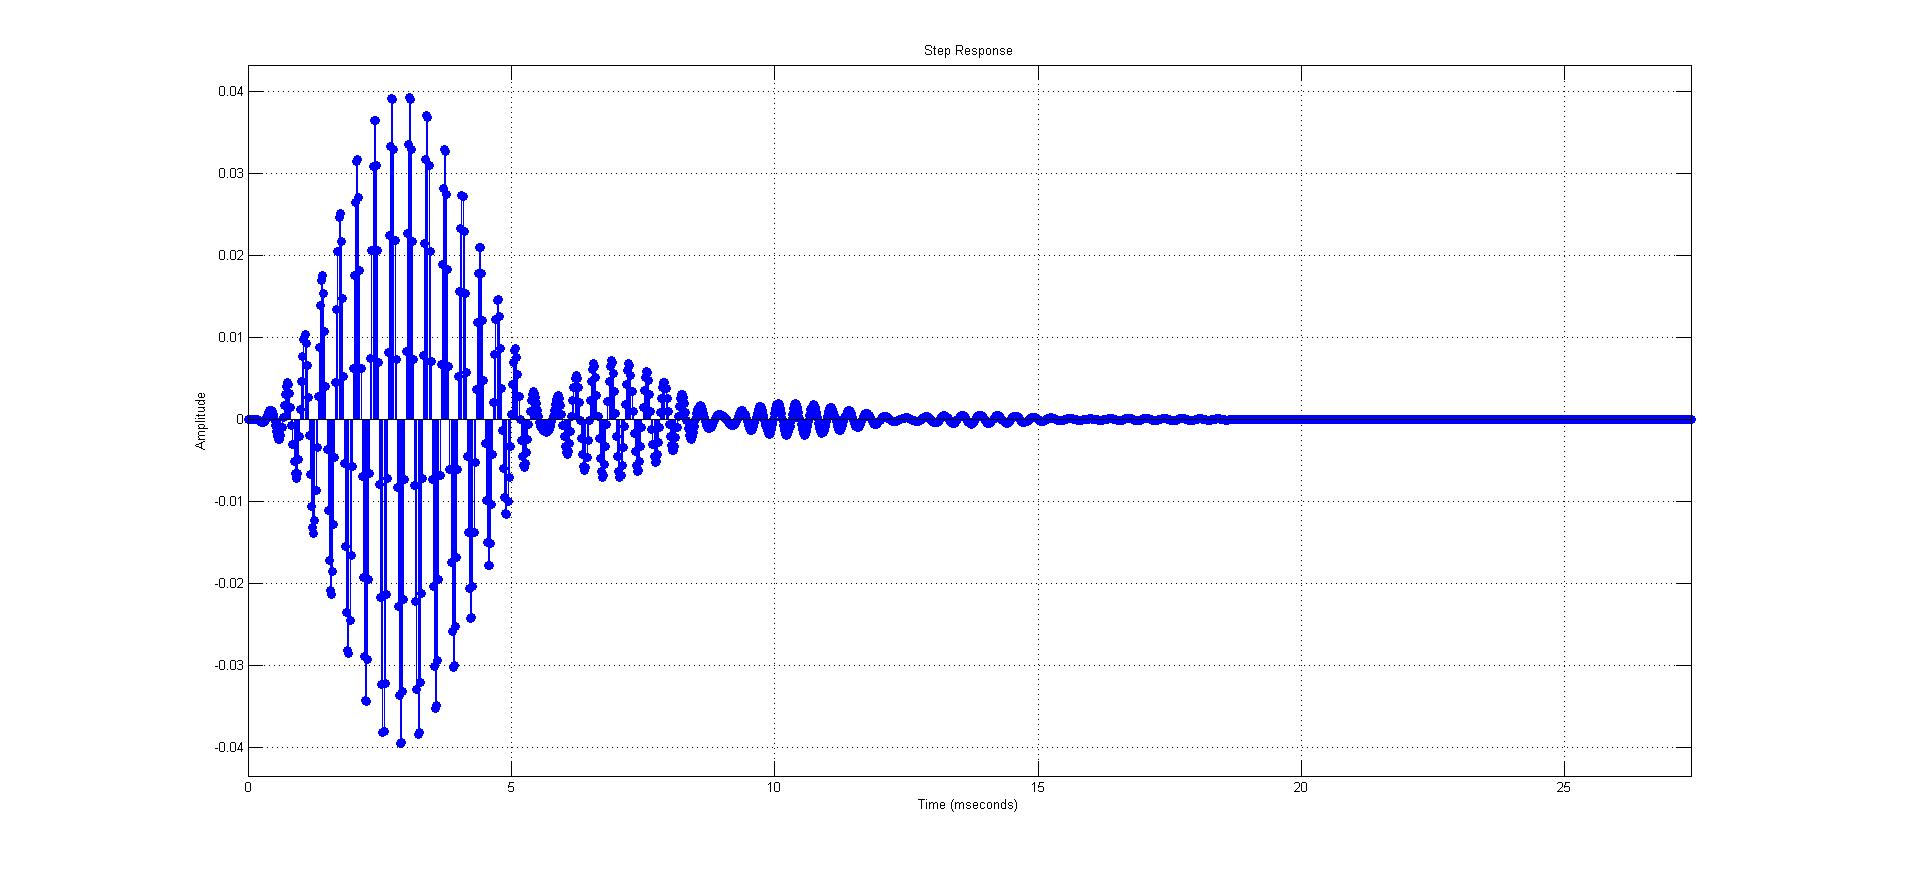
\includegraphics[width=\textwidth]{SprungantwortIdeal.png}
  \caption{Ideale Sprungantwort des Filters}
  \label{fig:SprungBandIdeal}
\end{figure}
\begin{figure}[H]
  \centering
    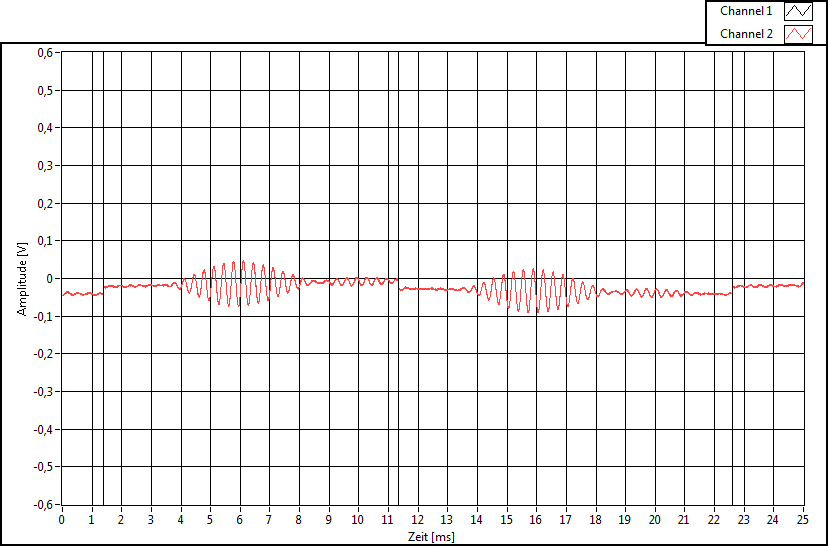
\includegraphics[width=\textwidth]{SprungantwortZoomReal.png}
  \caption{Reale Sprungantwort des Filters}
  \label{fig:SprungBandReal}
\end{figure}

In Abbildung \ref{fig:SprungBandIdeal} ist die Ideale Sprungantwort und in Abbildung \ref{fig:SprungBandReal} die Reale Sprungantwort des Filters zu sehen.
Beide Sprungantworten gleichen sich weites gehend. Die Amplituden der beiden Sprungantworten unterscheiden sich leicht, denn der reale Sprung ist bei uns ein Rechteck, welches eine Amplitude von \begin{math} V_{pp} = 2V \end{math} hat wohingegen der ideale Sprung nur eine Amplitude von \begin{math} V_{pp} = 1V \end{math} besitzt. Dies erklärt die leicht kleinere Amplitude der idealen Sprungantwort.\\ Ein weiterer Unterschied, ist die leichte Dämpfung auf dem Gleichspannungsanteil. Dies erklärt sich durch die Dämpfung des Systems.

\begin{figure}[H]
  \centering
    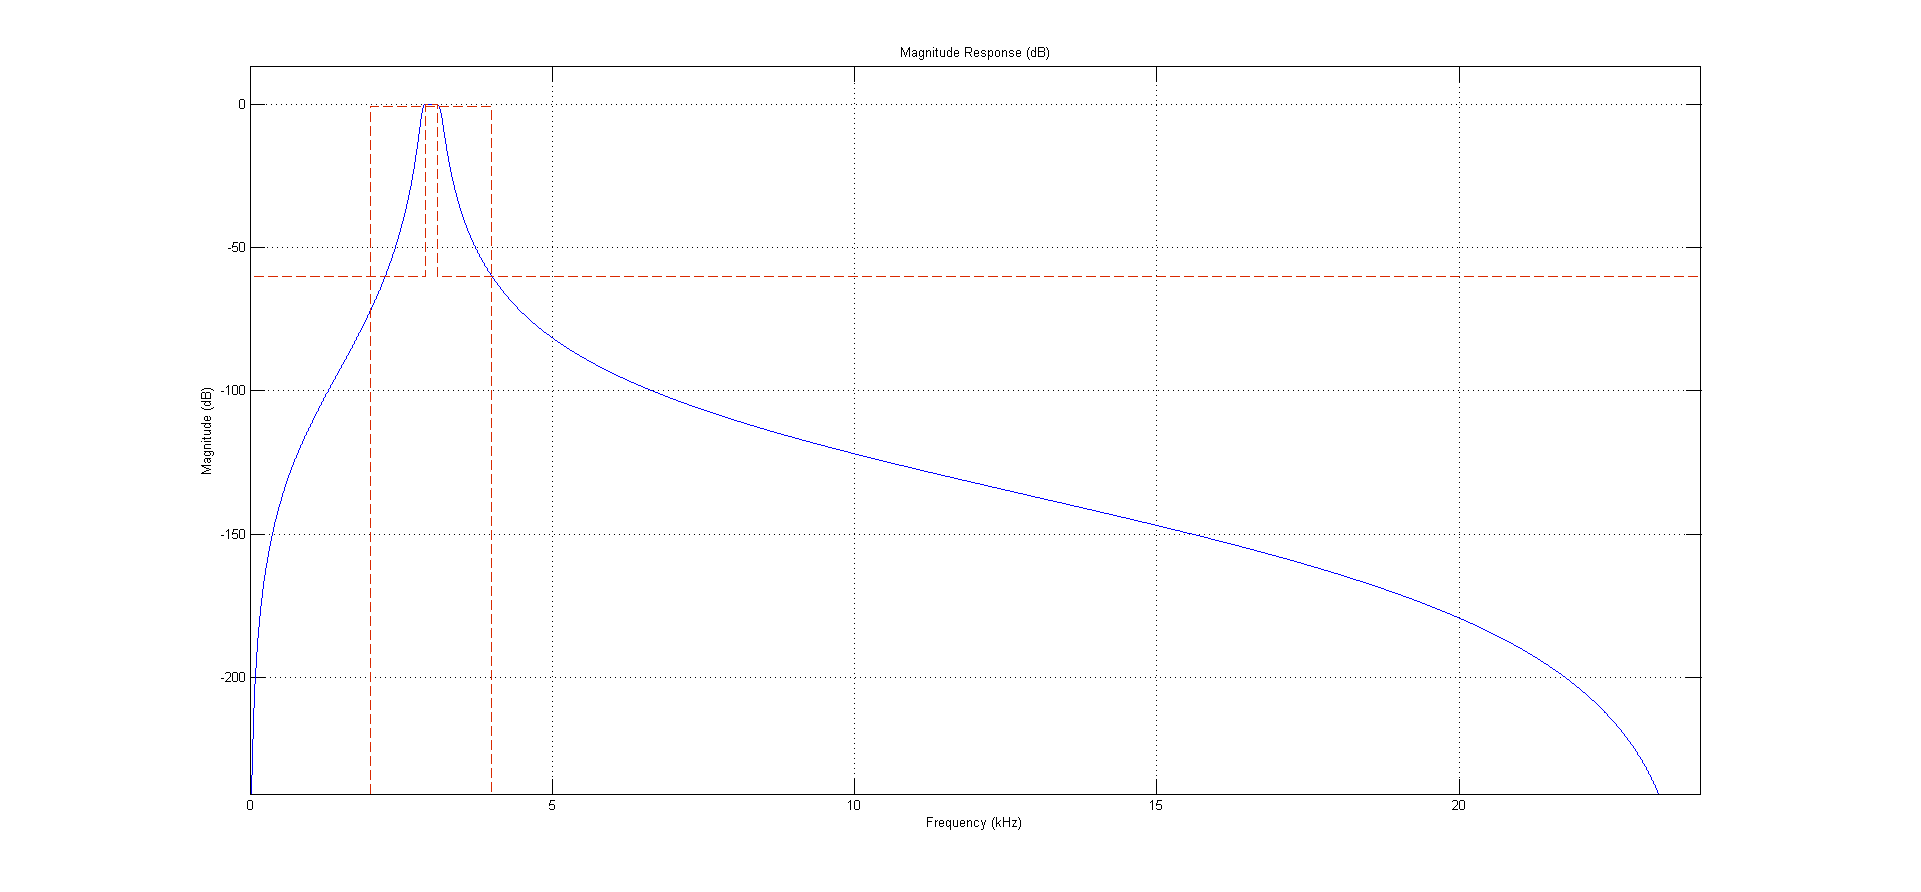
\includegraphics[width=\textwidth]{AmplitudengangIdeal.png}
  \caption{Idealer Amplitudengang des Filters}
  \label{fig:AmpBandIdeal}
\end{figure}
\begin{figure}[H]
  \centering
    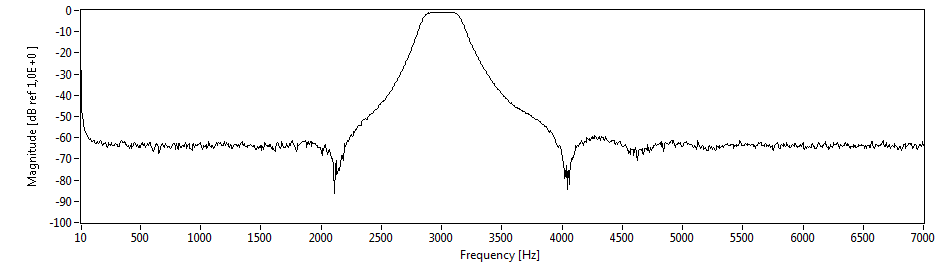
\includegraphics[width=\textwidth]{AmplitudengangReal.png}
  \caption{Realer Amplitudengang des Filters}
  \label{fig:AmpBandReal}
\end{figure}

Abbildung \ref{fig:AmpBandIdeal} ist der ideale Amplitudengang und in Abbildung \ref{fig:AmpBandReal} der reale Amplitudengang zu sehen. 
Beide Amplitudengänge sind sich ähnlich, weisen allerdings im Detail gravierende Unterschiede auf.
So erreicht der Reale Filter kein 0dB Dämpfung an der Passfrequenz sondern hat eine Dämpfung von 1dB, dies ist die Dämpfung des Systems. Außerdem wird in den Stoppbändern keine Dauerhafte Dämpfung von unter 60dB erreicht. Dies liegt ebenfalls am System, da dieses 10 Bit nutzt und dabei
0 dB bis -60 dB bei einer Auflösung von 1 dB darstellt. Allerdings erfüllt dies trotzdem die Anforderung.
